\section{LEM - Lattice-Element-Method}
The lattice element method (LEM) is a well-known model for the simulation of the fracture in the cemented geomaterial and concrete. In comparison to the discrete element method (DEM), where the contact search and contact mechanics are implemented, the LEM represents the medium with a series of spring or beam elements to simulate the fracking process. The considered LEM in this study is fully developed in Kiel University (CAU Kiel) and is implemented in various engineering applications. In earlier studies, the application of LEM was restricted to fracture simulation in concrete, where the heterogeneity was introduced with defining the aggregates, mortar and interface bond zone \cite{Liuetal2007, Pradoetal2003, Vanmieretal2002}. With the development of LEM its application is extended to failure behavior of cemented geomaterials such as bio-cemented granular material \cite{Rizvietal2019a}. The LEM is also used to simulate the fracture under dynamic loading for the foam concrete \cite{Rizvietal2018a}, masonry walls \cite{Sattarietal2019a} and cemented geomaterial \cite{ Rizvietal2018c, Rizvietal2020a}. Figure \ref{fig:Amir_LEM_Code} depicts the coupled THM processes and affected geomaterial parameters, which are implemented in LEM algorithm.

\begin{figure}[!ht]
\centering
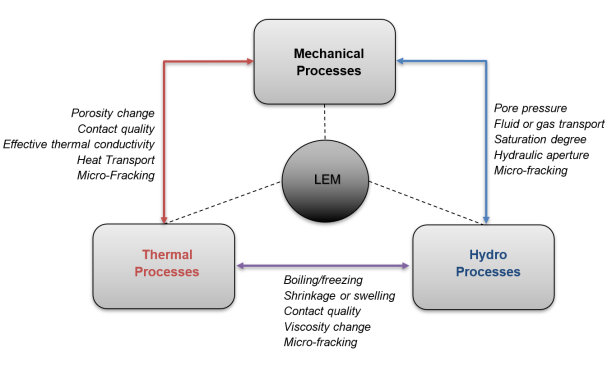
\includegraphics[width=12cm,height=7cm]{figures/Amir_LEM_Code.png}
\caption{The simulation of the coupled THM processes with LEM}
\label{fig:Amir_LEM_Code}
\end{figure} 

In its recent application, the evaluation of effective properties in shallow crustal rock is investigated \cite{Rizvietal2019c}. The developed in-house LEM model is applied for the simulation of the heat transfer in modified granular material and assessment of effective thermal conductivity \cite{Rizvietal2020b, Rizvietal2018b, Rizvietal2016, Shresthaetal2019} as well as the Nano geocomposites (\cite{Rizvietal2019d}). The thermo-mechanical LEM model is implemented to simulate the change of the thermal conductivity of the rocks under mechanical and thermal loadings \cite{Sattarietal2017}. With an integration of the interface element, the LEM is able to simulate the fully coupled TM processes in cemented geomaterial \cite{Sattarietal2019b}. The application of LEM is extended to model the hydro-mechanical processes \cite{Grassl2009, Grassletal2013}. In these models, the dual lattice setup is considered, where lattice elements transfer the mechanical loads between the nodes and conduct elements only carry the fluid flow. Similar to DEM models \cite{Simaetal2013}, the LEM is extended to simulate the shrinkage and swelling processes in rock material. In the scope of this study, the LEM is also used for the simulation of pressurized percolation tests in rock material. In this model, the mass conservation law is implemented and artificial cavities for fluid or gas transport are defined. In CAU Kiel, we are devoted to continue the development of the LEM and overcome its application limitations. In this sense, the parallel computing for computing efficiency is under process and development. The ongoing work incorporate the plasticity, visco-plasticity, flow, hardening, fatigue and creep rules to establish a constitutive lattice model, which can be implemented in the practical applications to simulate the geomaterial response under the coupled THM processes.\\





